% !TEX TS-program = xelatex
% !TEX encoding = UTF-8 Unicode

% Tennessee Technological University
% ME4140 - Fall 2016 - Fall 2017 - Fall 2020 
% Tristan Hill - September 10, 2020
% Module 5 - Turtlebot Family


\documentclass[fleqn]{beamer} % for presentation (has nav buttons at bottom)

\usepackage{/home/thill/Documents/lectures/cpp_workshop/modules/cpp_lectures}

\newcommand{\MNUM}{0\hspace{2mm}} % Module number
\newcommand{\TNUM}{---\hspace{2mm}} % Topic number - single topic for now
\newcommand{\moduletitle}{Introduction to C++} % Titles and Stuff
%\newcommand{\topictitle}{---} 

\newcommand{\sectiontitleI}{Course Structure} % More Titles and Stuff
\newcommand{\sectiontitleII}{Course Topics - Learning Objectives}
\newcommand{\sectiontitleIII}{Anatomy of A Computer}
\newcommand{\sectiontitleIV}{The C++ Programming Language}
\newcommand{\sectiontitleV}{Tutorial 1 - Hello World}

\setbeamercolor{title in head/foot}{fg=TTUgold} % this needs work...


\title{GSET - Programming with Mr. Hill}
\author{Tristan Hill\vspc \hspc Tennessee Technological University \hspc}
\date{Summer 2021}


\begin{document}

\lstset{language=MATLAB,basicstyle=\ttfamily\small,showstringspaces=false}

\frame{\titlepage \center\begin{framed}\Large \textbf{Module \MNUM - \moduletitle}\end{framed} \vspace{5mm}}

% Section 0 - Outline
\frame{
	
	\large \textbf{Module \MNUM - \moduletitle} \vspace{3mm}\\
	
	\begin{itemize}
	
		\item \hyperlink{sectionI}{\sectiontitleI} \vspc % Section I
		\item \hyperlink{sectionII}{\sectiontitleII} \vspc % Section II
		\item \hyperlink{sectionIII}{\sectiontitleIII} \vspc %Section III
		\item \hyperlink{sectionIV}{\sectiontitleIV} \vspc %Section IV	
		\item \hyperlink{sectionV}{\sectiontitleV} \vspc %Section V
	
	\end{itemize}

}

\section{\sectiontitleI}

	% Section I - Frame I
	\begin{frame}[label=sectionI,containsverbatim] \small
		\frametitle{\sectiontitleI}
		\underline{\large Lectures and Assignments}
		\begin{itemize}
			\item This programming course is organized into topic based modules. Each module contains a lecture with slides, and a tutorial with instructions and example code.  
			
			\item The lectures will be held in class, and after each lecture we will work on the tutorials as a group. After completing each tutorial you will write a short summary (README) documenting your program and the work you have done.
			
			\item In addition to the tutorials, programming challenges will be assigned throughout the course to test the skills you have acquired. After completing each programming assignment you will write a short report documenting your program and the work you have done.  
		\end{itemize}
	\end{frame}

	% Section I - Frame II
	\begin{frame} \small
		\frametitle{\sectiontitleI}
		\underline{\large Exams and Grading}	
		\begin{itemize}
			\item You will take a midterm and a final exam in class, and each exam will have a paper and programming component.
			
			\item Your final grade comes from participation in the tutorials (25\%), completion of the programming challenges(25\%), as well as the two graded exams (25\% + 25\%).     
			
			\item See the published syllabus for the complete course details and policies. 
			
		\end{itemize}	
	\end{frame}

	% Section I - Frame III
	\begin{frame} \small
		\frametitle{\sectiontitleI}
		\underline{\large Collaboration and Group Work}	
		\begin{itemize}
			\item Discussion between peers and the instructors is encouraged for all assignments except during the exams.
			
			\item Some assignments may be completed as a group, but some must be completed as individuals. Ask the instructor if you are unsure. 
			
			\item {\BL Sharing of code between students or is \underline{not allowed} unless the activity is designated as a group assignment by the instructor. \vspace{2mm} \\ The Tennessee Technological University academic misconduct policy clearly states that all submitted work must be original and authored by the student(s) submitting the assignment.} 		
		\end{itemize}	
	\end{frame}



\section{\sectiontitleII}

	% Section II - Frame I
	\begin{frame}[label=sectionII,containsverbatim] \small
		\frametitle{\sectiontitleII}
 		During this course we are going to learn about structured computer programming and the C++ Language. The following topics will be covered.
		\begin{itemize}
			
			\item Variables, Expressions, and Assignment
			
			\item Basic Input and Output Operations
			
			\item Computer Memory and Common Data Structures
			
			\item Logic and Selection Statements 
			
			\item Looping and Iteration 
			
			\item Introduction to Object Oriented Programming  
			
		\end{itemize}


	\end{frame}

\section{\sectiontitleIII}

	% Section II - Frame I
	\frame{ \small
		\frametitle{\sectiontitleIII}
		
		\underline{\large Major Components}
		\begin{itemize}
			
			\item
			\item 
			\item 
			\item  
			\item
			\item	
			
		\end{itemize}
	}

\section{\sectiontitleIV}	
	% Section IV - Frame I
	\begin{frame}[label=sectionIV] \small
		\frametitle{\sectiontitleIV}    
		
		\underline{A Few Questions}
		\setbeamertemplate{itemize items}[triangle]
		\begin{itemize}
			
			\item What is a computer program? What is computer programming?
			
			\item Have you ever learned about programming before? If so what languages did you use, and where did you learn about them? What types of problems did you solve?
			
			\item Have you ever learned about C++? Why is C++ important for scientists and engineers? 
				\begin{itemize}
					\item 
					\item
					\item
				\end{itemize}
			
			
		\end{itemize}
	\end{frame}

\section{\sectiontitleV}	
	% Section V - Frame I
	            \begin{frame}[label=sectionV] \small
		\frametitle{\sectiontitleV}    
	
 \setbeamertemplate{itemize items}[triangle]
                \begin{itemize}

					\item {\bf Overview:} In the first tutorial you are going to choose your programming environment on your computer and write your first program, {\it Hello World}.  		

					\item {\bf Assignment:} Complete the tutorial in the document {\it tutorial\MNUM\_introduction\_cpp.pdf } on ilearn. You must be able to display a custom message from your program to the the terminal or standard output.
                    
                    \item {\bf Deliverable:} Write a brief summary of what you accomplished and what you struggled with the most. Include a screen shot or copy of the output of your program.   
    
                    \item {\bf Next Week:} After completion of Module \MNUM, you are ready to learn about Variables, Expressions and Assignment. \vspc
                    
       
                \end{itemize}
		\end{frame}

\end{document}


%
%\begin{description}
%
%    \item [I. Components] The major building blocks of a ROS system
%
%        \begin{enumerate}
%                
%            \item \href{http://wiki.ros.org/Master}{Master Node}
%                \begin{itemize}
%                    \item {\it The ROS Master provides naming and registration services to the rest of the nodes in the ROS system.}** 
%                    \item master node runs first  {\fontfamily{qcr}\selectfont  \hspace{5mm} \$ roscore } \\
%                    \item core of the system or robot {\fontfamily{qcr}\selectfont  \hspace{5mm} \$ ROS\_MASTER\_URI=http://12345 } \\
%                    
%
%                \end{itemize}
%            
%            \item \href{http://wiki.ros.org/Nodes}{Nodes}             
%                \begin{itemize}
%                    \item {\it A node is a process that performs computation.}** 
%                    \item each 'program' or 'element' of the robot is a node\\examples:
%                        \begin{itemize} 
%                        \begin{multicols}{2}    
%                        
%                            \item sensor
%                            \item hardware driver    
%                            \item navigation 
%                            \item keyboard or joystick        
%                            
%                        \end{multicols}
%                        \end{itemize}
%                    \item start or run node individually after master\vspace{5mm}\\
%                    {\fontfamily{qcr}\selectfont  \hspace{5mm} \$ rosrun <packagename> <nodename> <options> } \vspace{1mm}\\
%                  
%                    \item all nodes are registered to the master and communicate in different ways
%                        \begin{itemize}
%                            \item  \href{http://wiki.ros.org/Topics}{topics} - publishing and subscribing
%                            \item \href{http://wiki.ros.org/Parameter%20Serverparameters}{parameter server} - static data
%                            \item \href{http://wiki.ros.org/Services}{services} - subroutine call
%                        \end{itemize}    
%                                      
%                \end{itemize}
%                
%            \item \href{http://wiki.ros.org/Packages}{Packages} 
%
%                \begin{itemize}
%                    \item {\it Software in ROS is organized in packages. A package might contain ROS nodes, a ROS-independent library, a dataset, configuration files, a third-party piece of software, or anything else that logically constitutes a useful module.}** 
%                    \item a collection of related nodes, each node belongs to a package
%                                     
%                    \item pre-built packages available with ros installation {\fontfamily{qcr}\selectfont  \hspace{5mm} -desktop-full}
%                    \item pre-built packages available for installation \\
%                    \begin{description}
%                        \item[apt] {\fontfamily{qcr}\selectfont  \hspace{1mm} \$ sudo apt-get install ros-<distribution>-<packagename> } 
%                        \item[rosdep]{\fontfamily{qcr}\selectfont  \hspace{1mm} \$ rosdep install <packagename> } \\
%                    \end{description}
%                    \item update ubuntu before installing anything \\
%                    {\fontfamily{qcr}\selectfont  \hspace{2mm} \$ sudo apt-get update } \\
%                    {\fontfamily{qcr}\selectfont  \hspace{2mm} \$ sudo apt-get check }                
%                \end{itemize}            
%
%                
%                
%    \end{enumerate}
%    ** from (ros.org)
%    \newpage
%    
%    \item [II. The Graph of the System] ROS works on a system of interconnected nodes. It is very useful to visualize this in a graph.\\
%        \begin{enumerate}   
%            
%            \item \href{http://wiki.ros.org/rqt_graph}{RQT Graph} A very useful tool. A node {\it rqt\_graph} in a package {\it rqt\_graph}. \\\\
%                    {\fontfamily{qcr}\selectfont  \hspace{5mm} \$ rosrun rqt\_graph rqt\_graph}\\
%            
%            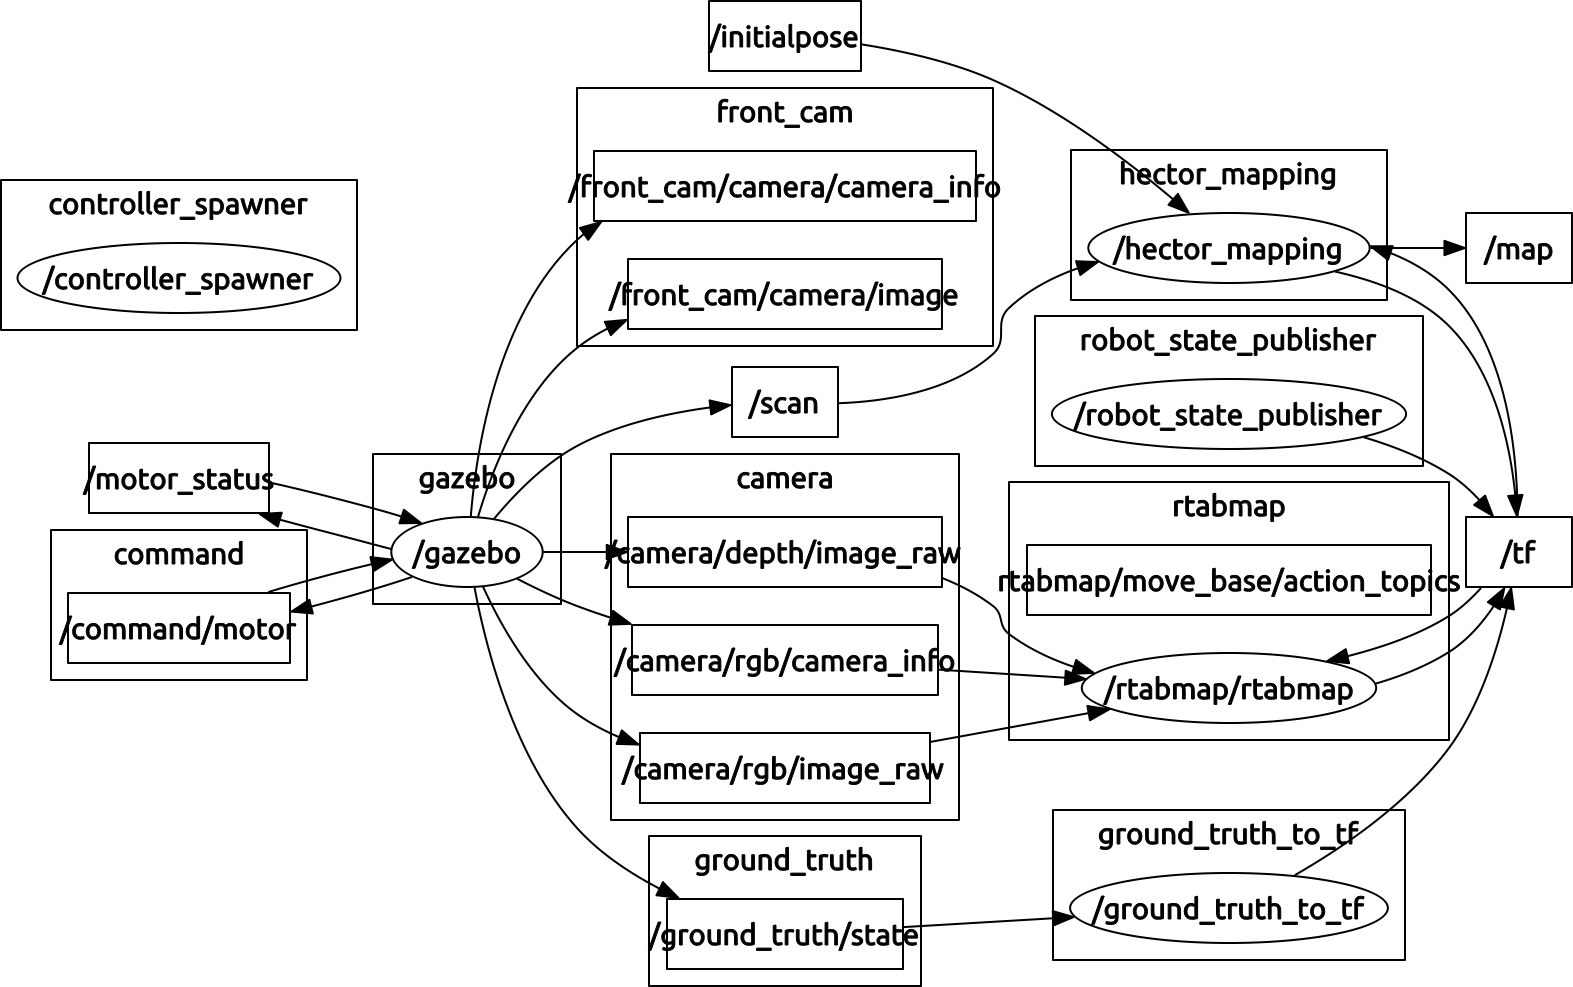
\includegraphics[scale=.4]{ros_basics_fig1.png} \\
%            
%            \item \href{http://wiki.ros.org/rqt_plot}{RQT Plot} A very useful tool. A node {\it rqt\_plot} in a package {\it rqt\_plot}. \\
%                {\fontfamily{qcr}\selectfont  \hspace{5mm} \$ rosrun rqt\_plot rqt\_plot}\\
%            
%            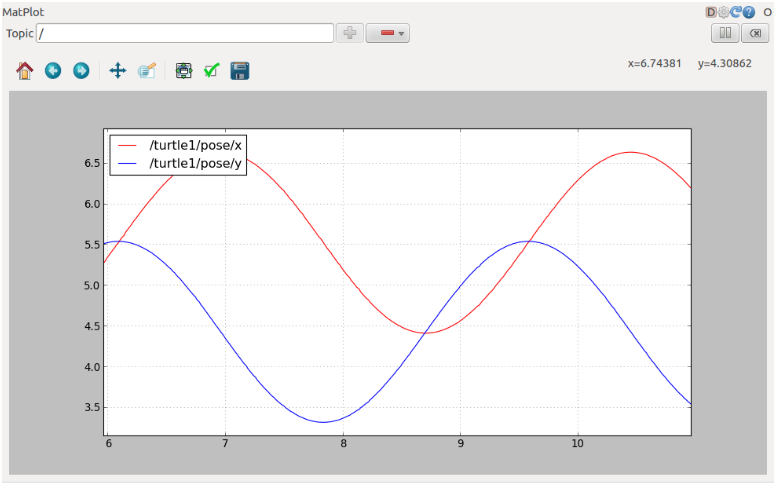
\includegraphics[scale=.5]{ros_basics_fig2.png} \\    
%          \end{enumerate}       
%
%
%\newpage
%    
%    \item [III. Topics, Publishers, and Subscribers] The nodes in a ROS system communicate.  
%        \begin{enumerate}   
%           \item \href{http://wiki.ros.org/Topics}{Topics} 
%                    \begin{itemize}
%                        \item data available to nodes in the system
%                        \item each topic has a name    
%                        \item data is stored and transferred in standard ros data types
%                        \item generally data is streaming, but does not have to be
%                    \end{itemize}    
%           \item \href{http://wiki.ros.org/ROS/Tutorials/WritingPublisherSubscriber(c++)}{Publishers}
%                    \begin{itemize}
%      
%                        \item data produced by a node can be shared with the system by publishing a topic
%                        \item a node which outputs topic data is a publisher
%                        \item a node may publish multiple topics 
%                        
%                        \end{itemize}  
%            \item \href{http://wiki.ros.org/ROS/Tutorials/WritingPublisherSubscriber(c++)}{Subscribers}
%                \begin{itemize}
%      
%                        \item a registered node can access the data in a topic by subscribing to a topic
%                        \item a node which gets topic data as input is a subscriber
%                        \item a node may subscribe to multiple topics 
%                    \end{itemize}  
%                    
%            \item \href{http://wiki.ros.org/rostopic}{rostopic}                    
%                \begin{itemize}   
%                    \item a very useful tool, a built in package 
%                    \item used differently than other packages, does not require rosrun
%                    \item a set of different tools
%                    \begin{description}   
%                        \item [list] {\fontfamily{qcr}\selectfont  \hspace{5mm} \$ rostopic list}\\
%                        \item [echo] {\fontfamily{qcr}\selectfont  \hspace{5mm} \$ rostopic echo /topicname}\\
%                        \item [type] {\fontfamily{qcr}\selectfont  \hspace{5mm} \$ rostopic pub /topicname}\\
%                    \end{description}  
%                \end{itemize}    
%                    \item  \href{http://wiki.ros.org/msg}{data types} - topics are published in standard types called messages
%                    \begin{itemize}
%                        \item {\fontfamily{qcr}\selectfont  \hspace{5mm} std\textunderscore msgs/int32 }
%                        \item {\fontfamily{qcr}\selectfont  \hspace{5mm} std\textunderscore msgs/float32 }\\
%                        
%                        \item {\fontfamily{qcr}\selectfont  \hspace{5mm} geometry\textunderscore msgs/Point }
%                        \item {\fontfamily{qcr}\selectfont  \hspace{5mm} geometry\textunderscore msgs/Pose }\\
%                        
%                        \item {\fontfamily{qcr}\selectfont  \hspace{5mm} nav\textunderscore msgs/Odometry }
%                        \item {\fontfamily{qcr}\selectfont  \hspace{5mm} nav\textunderscore msgs/Path }\\
%                    \end{itemize}
%                    
%                    \item let show an example now!
%                                      
%        \end{enumerate}     
%\newpage
%    
%%    \item [IV. Services] The nodes in a ROS system can also communicate through services. Thsi is for reply/request type operations.  
%%  \begin{enumerate} 
%%\item \href{http://wiki.ros.org/Services}{Services}
%%\end{enumerate}    
%%\newpage
%    
%
%\end{description}
%\end{document}
%
